\documentclass[spanish]{beamer}
\usepackage[ansinew]{inputenc} % Acepta caracteres en castellano
\usepackage[spanish]{babel}    % silabea palabras castellanas
\usepackage{amsmath}
\usepackage{mathtools,cancel} % cancela con una flecha \cancelto{0}{XXXX}
\renewcommand{\CancelColor}{\color{red}} %change cancel color to red
\usepackage{amsfonts}
\usepackage{amssymb}
\usepackage{dsfont}
\usepackage{graphicx}
\usepackage{geometry}
\usetheme{Madrid}
\usecolortheme{beaver}
\usepackage{textpos}
% Logo  en el comienzo 
\addtobeamertemplate{frametitle}{}{%
\begin{textblock*}{100mm}(.85\textwidth,-1cm)
{\includegraphics[height=0.4in, keepaspectratio=true]{/Users/luisnunez/Dropbox/MisDocumentos/UIS/UISImagenInstitucional/UISLOGO.png}}
\end{textblock*}}

\begin{document}

\title{\textbf{T�tulo presentaci�n} }
\author[L.A. N��ez]{\textbf{Luis A. N��ez}}  
\institute[UIS]{\textit{Escuela de F�sica, Facultad de Ciencias, } \\
\textit{Universidad Industrial de Santander, Santander, Colombia } \\
{\includegraphics[height=0.4in, keepaspectratio=true]{/Users/luisnunez/Dropbox/MisDocumentos/UIS/UISImagenInstitucional/UISLOGO.png}}
}
\date{\today}
\maketitle


\begin{frame}
\frametitle{Agenda}
  \tableofcontents
\end{frame}


%%%%% Diapo 1
\section{Hamiltoniano y P�ndulo}
\subsection{El problema y las coordenadas}
\frame{
  \frametitle{Hamiltoniano y P�ndulo}
El punto de suspensi�n de un p�ndulo est� obligado a moverse a lo largo de la par�bola $y=a x^2$. Encontrar el Hamiltoniano.
  \begin{figure}[t]
	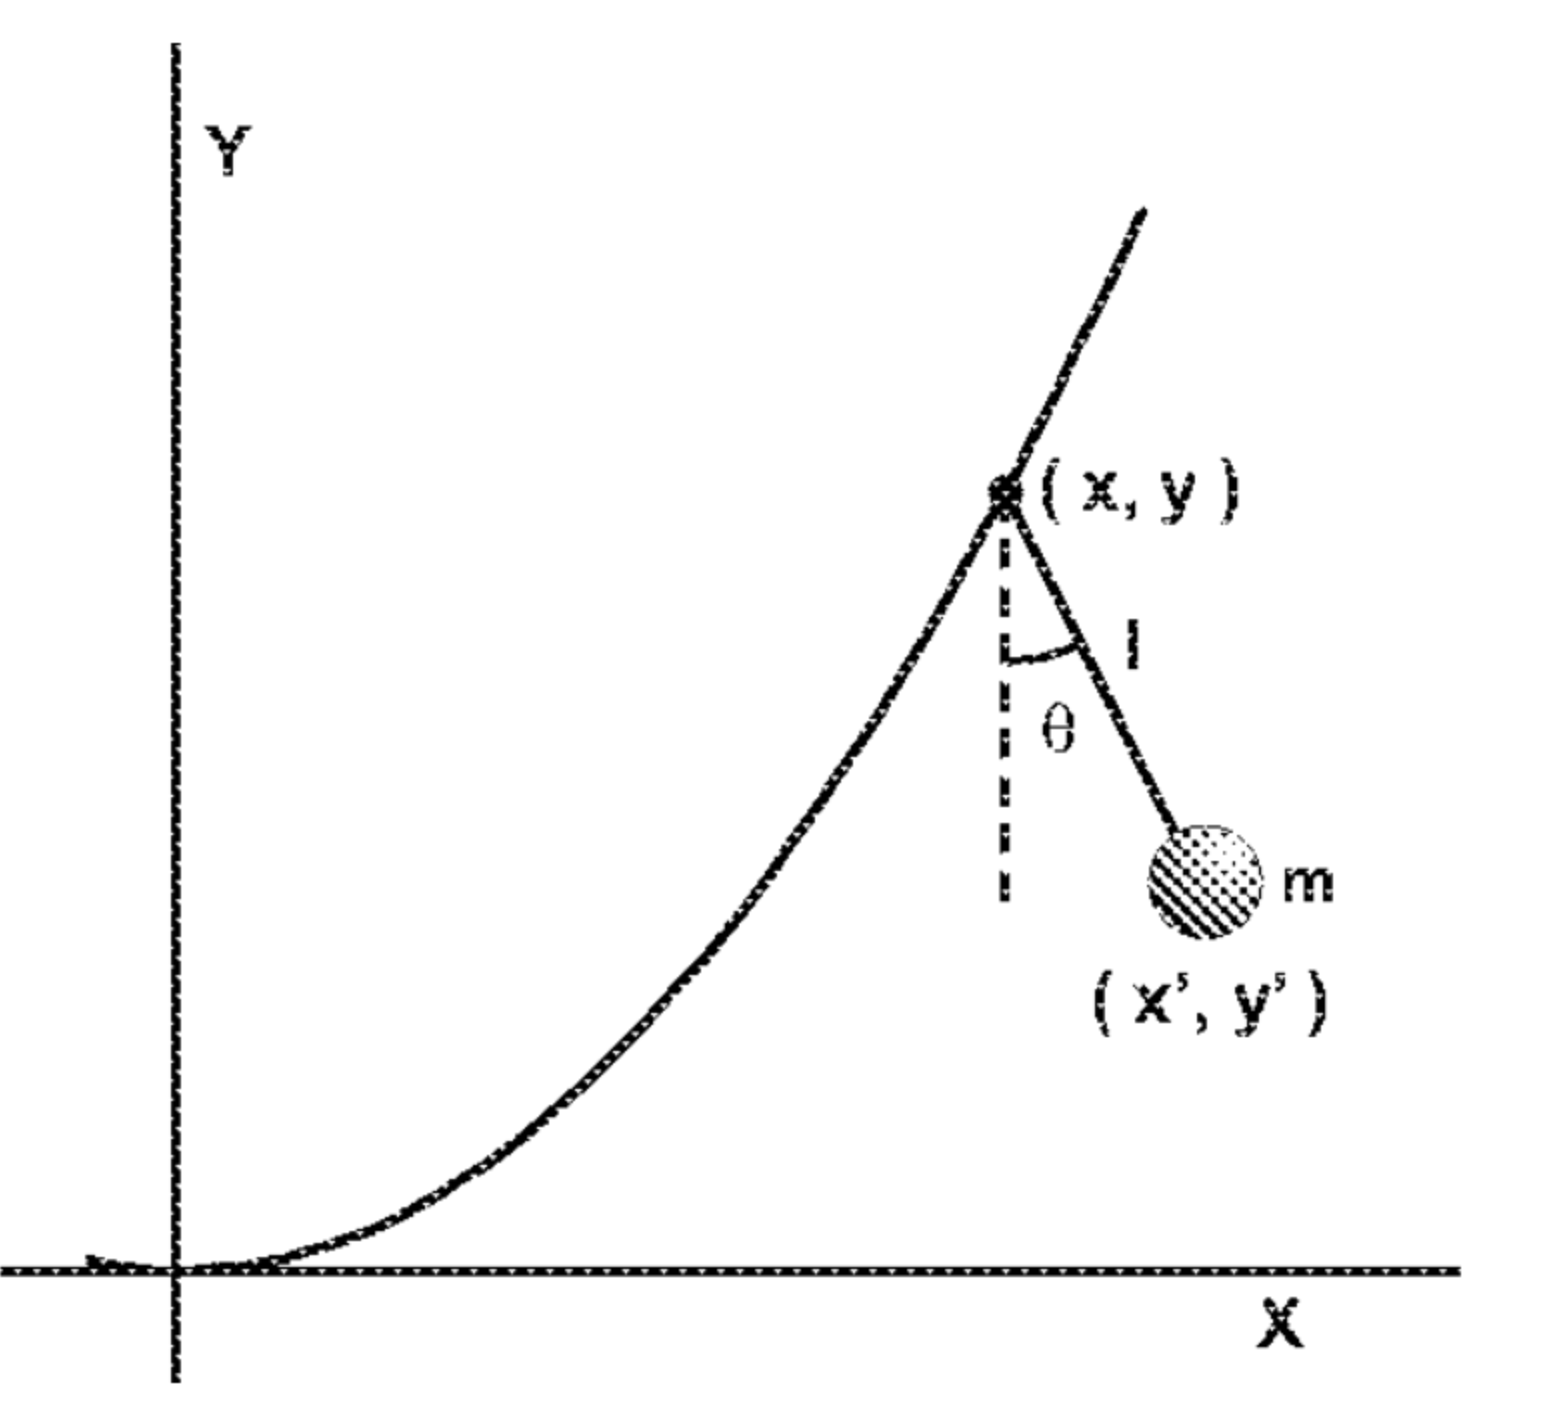
\includegraphics[width=1.8in]{Figuras/PenduloCurva.png}
   \end{figure}
   \begin{itemize}  
  	\item<1-> Sen las coordenadas del punto de sustentaci�n del p�ndulo son $x, y$ y las coordenadas de la masa $x^{\prime}, y^{\prime}$, 
	\item<2-> Se tiene las siguientes relaciones: $x^{\prime}=x+l \operatorname{sen} \theta, \quad y^{\prime}=y-l \cos \theta=a x^2-l \cos \theta$ \\
	$\dot{x}^{\prime}=\dot{x}+l \dot{\theta} \cos \theta, \quad \dot{y}^{\prime}=\dot{y}+l \dot{\theta} \operatorname{sen} \theta=2 a x \dot{x}+l \dot{\theta} \operatorname{sen} \theta$
    \end{itemize}
}
%
%%%%% Diapo 2
\subsection{El Lagrangeano y el Hamiltoniano}
\frame{
\frametitle{El Lagrangeano y el Hamiltoniano}
\begin{itemize}  
	\item<1-> La energ�a cin�tica viene dada por: 
	$ T  =\frac{1}{2} m\left(\dot{x}^{\prime 2}+\dot{y}^{\prime 2}\right) \Rightarrow$ $T =\frac{1}{2} m\left(\dot{x}^2+l^2 \dot{\theta}^2+4 a^2 x^2 \dot{x}^2+2 l \dot{x} \dot{\theta} \cos \theta+4 a x l \dot{x} \dot{\theta} \operatorname{sen} \theta\right)$
	\item<2-> y la energ�a potencial por: $V=m g y^{\prime}=m g\left(a x^2-l \cos \theta\right)$
	\item<3-> A partir del lagrangiano $\mathcal{L}=T-V$, obtenemos 
	$p_x  =\frac{\partial L}{\partial \dot{x}}=m \dot{x}\left(1+4 a^2 x^2\right)+m l \dot{\theta}(\cos \theta+2 a x \operatorname{sen} \theta)$ 
	$p_\theta  =m l^2 \dot{\theta}+m l \dot{x}(\cos \theta+2 a x \operatorname{sen} \theta)$
	\item<4-> Despejando las velocidades
	$\dot{x} =\frac{p_x}{m} \frac{1}{(\operatorname{sen} \theta-2 a x \cos \theta)^2}-\frac{p_\theta}{m l} \frac{\cos \theta+2 a x \operatorname{sen} \theta}{(\operatorname{sen} \theta-2 a x \cos \theta)^2}$ 
	$\dot{\theta}  =\frac{p_\theta}{m l^2} \frac{1+4 a^2 x^2}{(\operatorname{sen} \theta-2 a x \cos \theta)^2}-\frac{p_x}{m l} \frac{\cos \theta+2 a x \operatorname{sen} \theta}{(\operatorname{sen} \theta-2 a x \cos \theta)^2}$
	\item<5-> Con lo cual 
	$\mathcal{H}  =\dot{x} p_x+\dot{\theta} p_\theta-L$ se puede expresar \\
	$\mathcal{H} =\frac{p_x^2}{2 m} \frac{1}{(\operatorname{sen} \theta-2 a x \cos \theta)^2}+\frac{p_\theta^2}{2 m l^2} \frac{1+4 a^2 x^2}{(\operatorname{sen} \theta-2 a x \cos \theta)^2}$
\end{itemize}
}

%
%%%%% Diapo 2
\section{$\mathcal{H}=q+t e^p$ y la transformaci�n $Q=q+e^{p}, P=p$}
\frame{
\frametitle{$\mathcal{H}=q+t e^p$ y $Q=q+e^p \quad \& \quad P=p$ 1/2}
El hamiltoniano de un cierto sistema f�sico es: $\mathcal{H}=q+t e^p$. Muestre que la transformaci�n $Q=q+e^p, P=p$ es una transformaci�n can�nica. Seguidamente, encuentre la funci�n generatriz de esta transformaci�n. Finalmente, determine el nuevo hamiltoniano y resuelva las ecuaciones de movimiento en las nuevas coordenadas.\\ 
$\cdot$ \\
Para determinar si la transformaci�n es can�nica, construimos el par�ntesis de Poisson entre las coordenadas
	como $\{f, g\} = \frac{\partial f}{\partial q} \frac{\partial g}{\partial p} - \frac{\partial f}{\partial p} \frac{\partial g}{\partial q}$, entonces: 
\begin{itemize}  
	\item<1-> $\{Q, Q\} = \frac{\partial Q}{\partial q} \frac{\partial Q}{\partial p} - \frac{\partial Q}{\partial p} \frac{\partial Q}{\partial q} = (1)(e^p) - (e^p)(1) = 0$;
	\item<2-> $\{P, P\} = \frac{\partial P}{\partial q} \frac{\partial P}{\partial p} - \frac{\partial P}{\partial p} \frac{\partial P}{\partial q} = (0)(1) - (1)(0) = 0$; y finalmente
	\item<3-> $\{Q, P\} = \frac{\partial Q}{\partial q} \frac{\partial P}{\partial p} - \frac{\partial Q}{\partial p} \frac{\partial P}{\partial q}$. Calculando cada una
	$\frac{\partial Q}{\partial q} = 1$, $\frac{\partial Q}{\partial p} = e^p$, $\frac{\partial P}{\partial q} = 0$, y $\frac{\partial P}{\partial p} = 1$, obtenemos $\{Q, P\} = (1)(1) - (e^p)(0) = 1$.  
	\item<4-> Por lo tanto, como la tranformaci�n cumple con 
	$\{Q, Q\} = 0, \quad \{P, P\} = 0, \quad \text{y} \quad \{Q, P\} = 1$. {\bf Es can�nica}
\end{itemize}
}

%
%%%%% Diapo 2
%\section{Secci�n}
\frame{
\frametitle{$\mathcal{H}=q+t e^p$ y $Q=q+e^p \quad \& \quad P=p$ 2/2}
Para encontrar la funci�n generadora $ F $ supondremos una funci�n generadora del tipo $F_2(q, P)$, que depende de  $q$ y  $P$
\begin{itemize}  
	\item<1-> Las relaciones para \( F_2(q, P) \) son: $p = \frac{\partial F_2}{\partial q} \quad \text{y} \quad Q = \frac{\partial F_2}{\partial P}$
	\item<2-> Sustituyendo \( p = P \) en  $Q = q + e^P$, como \( Q = \frac{\partial F_2}{\partial P} \Rightarrow \), $ F_2(q, P) = qP + \int e^P \, dP \Rightarrow F_2(q, P) = qP + e^P + C$ y $\quad C= 0$
	\item<3->  La funci�n generadora es $F_2(q, P) = qP + e^P$
\end{itemize}
}

  
\end{document}
%
%%%%% Diapo 2
\section{Secci�n}
\frame{
\frametitle{T�tulo transparencia}
\begin{itemize}  
	\item<1-> 
\end{itemize}
}


	\begin{figure}[t]
		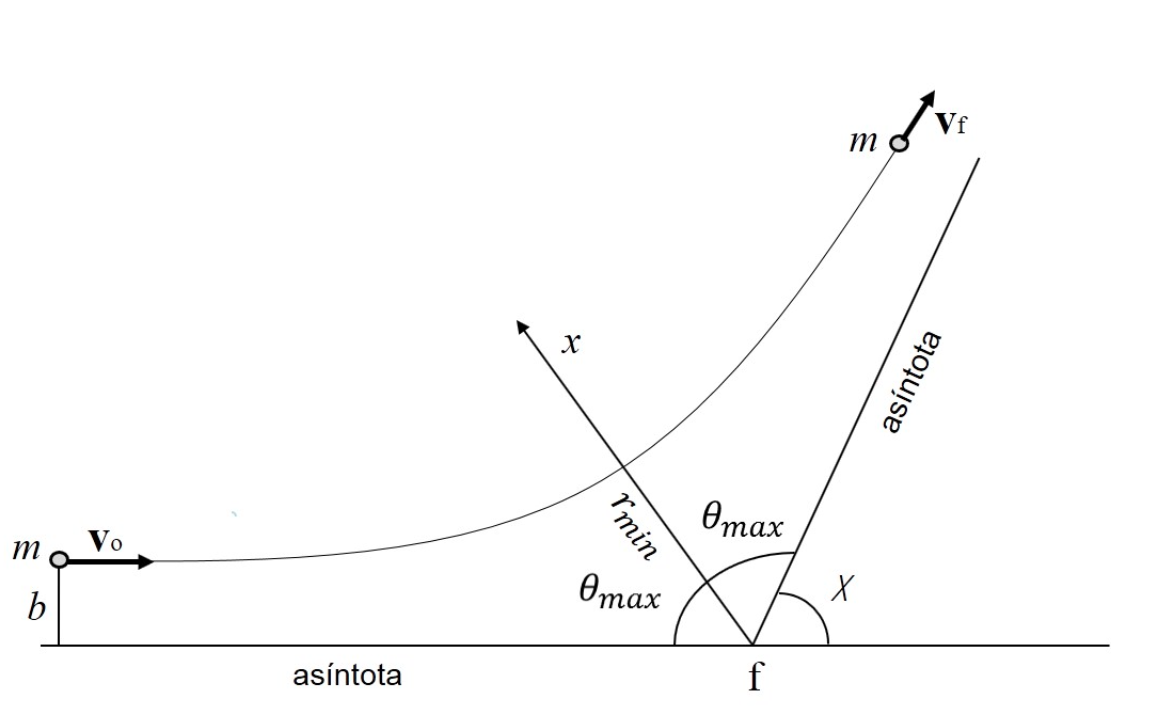
\includegraphics[width=1.8in]{Figuras/Dispersion.png}
   	\end{figure}
	
